\section{Semantic Segmentation}
\label{sec:SemanticSegmentation}

Semantic Segmentation models are used to create a mask of an image, in which every pixel is assigned to a class.
This method can be used to segment rails or rail tracks to obtain the direction of the train.

The first approach to filter out the rail tracks in front of the train was proposed by \cite{firstRailSegmentation2018} in 2018.
A SegNet \cite{SegNet2017} inspired network for semantic segmentation is extended with mixed pooling \cite{mixedPooling2014} and \ac{ASPP} from DeepLab \cite{deepLab2018}.
After the proposed semantic segmentation network outputs a binary mask with pixel labels being track or no track, a polygon fitting technique is utilized to refine the tracks further.
In 2019 \cite{railNet2019} introduced the RailNet architecture.
This model uses a ResNet-50 \cite{ResNet} backbone and a fully convolutional network \cite{FullyConvolutionalNetworks2015} to segment the rail tracks.
The network is designed in a pyramid structure \cite{FPN2017_two_stage-detector}, in which features of every ResNet stage are summed and up-sampled.
This combines low and high-level features, resulting in an enhanced performance.
\cite{railNet2019} reports higher accuracy than state-of-the-art segmentation models at the time with speeds up to 20 \ac{FPS} on an NVIDIA GTX1080 GPU.
Tests are made on the introduced \ac{RSDS} dataset further described in \autoref{subsubsec:RSDS}.

In 2019 RailSem19 \cite{railsem19dataset} introduced the first publicly available dataset for the rail domain.
This dataset also includes annotations for semantic segmentation tasks and experimented models like FRRNB \cite{FRRNBModel2017}.
This dataset is widely used in the community when working in the rail domain.
\cite{RailNet2020} already uses a subset of RailSem19 in 2020 and proposed another model named RailNet that uses a VGG16 \cite{VGGNet2015} backbone and an Information Aggregation Module.
Only rails are predicted, other annotations of RailSem19 are ignored.
The characteristics of rails like placement and structure are considered.
Therefore the integrated module is implemented to improve the spatial relationship between features on both the vertical and horizontal axes.
\cite{automatedSemSeg2022} uses four subsets of RailSem19 with 2, 3, 4, or all 19 classes to train the U-Net \cite{uNet2015} architecture.
Additionally, A cropping method is implemented to account for the difference in resolutions of RailSem19's images and the U-Net recommended one.
\cite{hadded2022application} used the RailSet dataset \cite{railSet2022}, which is an extension of RailSem19 for segmentation and anomaly detection tasks.
For details of the RailSet dataset please refer to \autoref{subsubsec:RailSet}.
U-Net \cite{uNet2015} and FRNN \cite{FRRNBModel2017} are trained with horizontal flips and zooming for the data augmentation.

In 2022 \cite{yuan2022railvid} proposed the RailVID dataset, which consists of infrared images instead of \ac{RGB} data to improve the system's abilities in challenging situations such as the absence of ambient light.
The dataset is described in \autoref{subsubsec:railVID} in more detail.
After collecting data, \cite{yuan2022railvid} experimented with widely used \ac{CNN}s for semantic segmentations, like \ac{CGNet} \cite{CGNet}, DeepLabv3+ \cite{DeepLabV3plus2018}, and \ac{BiSeNet} \cite{BiSeNet2019}.
Additionally, an improved BiSeNet architecture is proposed with consideration of the infrared data. Performance is enhanced by added layers to fuse low-level features.
In 2021 \cite{AccurateLightweightRailNet2021} proposed another architecture called RailNet.
It consists of an Encoder-Decoder structure incorporating depth-wise convolutions and a Segmentation Soul block, inspired by the context embedding block of \ac{BiSeNet}V2 \cite{BiSeNetV22021}.
Additionally, a port processing algorithm is utilized that is based on sliding window detection.
Tao et al. reports speeds up to 74 \ac{FPS} proving that this system is real-time capable \cite{AccurateLightweightRailNet2021}.

A topic that could be interesting is anomaly detection because many state-of-the-art approaches use semantic segmentation as a preprocessing step.
\cite{anomalyDetection2021} utilizes a \ac{BiSeNet} \cite{BiSeNet2019} architecture for segmenting rails, which is tailored for the anomaly detection task.
Therefore accuracy is preferred over speed.
While this network can detect small objects on the track, the system is not real-time capable.

\cite{RailraodSemanticPossibleTracks2020} is the first to consider a distinction between the trains own and adjacent tracks.
Consequently, the concept of "possible tracks" is introduced, which are all paths the train could follow under the assumption that the state of switches cannot be determined.
\autoref{fig:possibleTracks} visualizes this concept.
For detecting only the green tracks a U-Net-inspired \cite{uNet2015} semantic segmentation network is proposed, which incorporates a rule-based post-processing algorithm.
The network combines a ResNet-34 \cite{ResNet} backbone and includes connections to the upsampling blocks.
At the deepest level, a \ac{SPP} \cite{spatialPyramidPooling2014} and on the skip connections squeeze-and-excitation blocks \cite{SqueezeAndExcitation2019} are used.
Tests on RailSem19, show that it outperforms the first proposed RailNet \cite{railNet2019} in accuracy with a speed of 20 \ac{FPS}.

\vspace{0.5cm}

\begin{figure}[H]
    \centering
    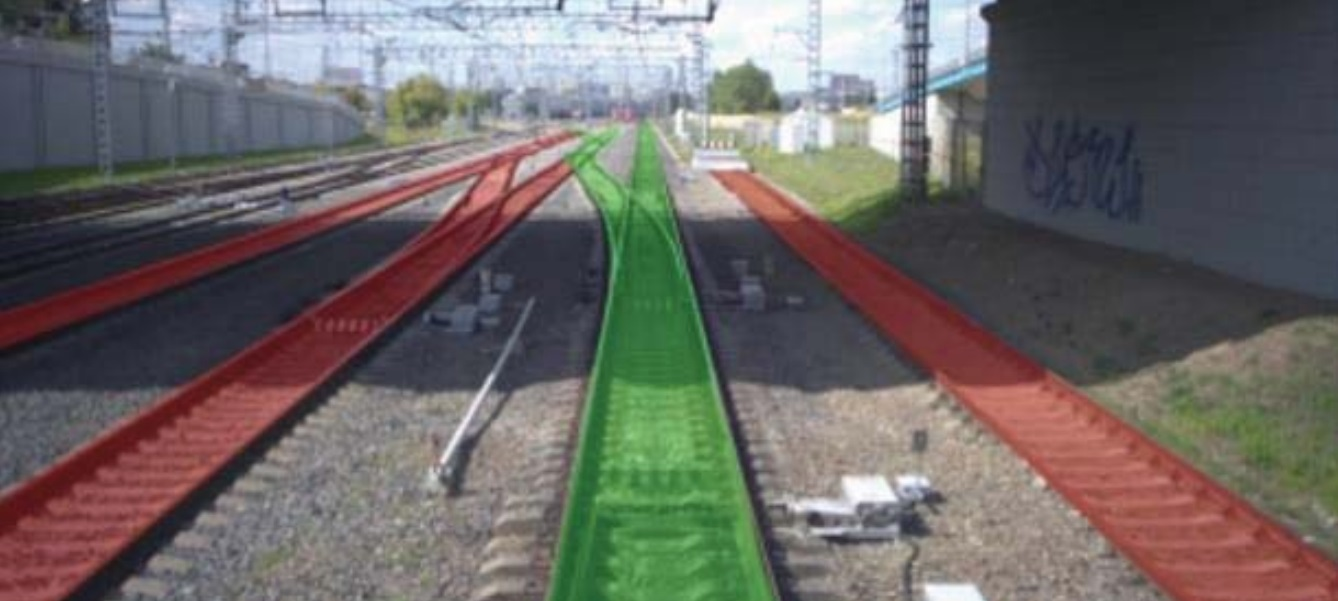
\includegraphics[width=0.5\linewidth]{PICs//semanticSegmentation/possibleTracks.jpg}
    \caption{Track segmentation in front of the train. Red are all adjacent tracks and green are possible tracks \cite{RailraodSemanticPossibleTracks2020}.}
    \label{fig:possibleTracks}
\end{figure}

\vspace{0.5cm}

In 2023 \cite{TPENet2023} further investigated the task of possible tracks and introduced \ac{TPE-Net}.
It consists of a DenseNet-inspired \cite{DenseNets} architecture, which is trained and tested on RailSem19 and outputs regressed heatmaps besides the segmented rails.
An example of such a heatmap is an image with one channel that shows the probability of each pixel being within a rail track.
The segmentation mask and the heatmaps are then used by a complex post-processing approach.
This process includes track point clustering, the creation of track segments, and the creation of a path tree, which is then used to generate all possible tracks.
Refinement is done by removing redundant paths and fitting polynomials.
Because of the complexity of this system, \cite{TPENet2023} reports speeds up to 12 \ac{FPS} making this system unsuitable for real-time applications.
Additionally, it is stated that problems arise when switches are present.


